\documentclass{article}
\usepackage{fancyhdr}
\usepackage{titlesec}
\usepackage{graphicx}
\graphicspath{ {./img/} }

\pagestyle{fancy}
\fancyhf{}
\lhead{Project UAS Praktikum Jaringan Komputer}
\rfoot{\footnotesize Page \thepage}
\lfoot{\footnotesize Mahyus Ihsan, S.Si, M.Si \newline Jurusan Informatika Universitas Syiah Kuala \newline Modul oleh : Diky Wahyudi, Furqan Al Ghifari, Rendika Rahmaturrizki}
\renewcommand{\headrulewidth}{1pt}
\renewcommand{\footrulewidth}{1pt}

\begin{document}
    \begin{center}
        \textbf{Build a Simple Office Network}
    \end{center}
	
	\begin{flushleft}
		 Anda ditugaskan untuk menyusun sebuah jaringan kantor sederhana. Kantor tersebut memiliki 4 buah ruangan yaitu \textbf{ruang printer}, \textbf{ruang server}, \textbf{ruang kerja bersama / tim}, dan \textbf{ruang kantor}. Perangkat untuk setiap ruangan adalah sebagai berikut :
	\end{flushleft}
   
    
	\begin{flushleft}
		Ruang Printer :
		\begin{itemize}
			\item 1 buah Printer
			\item 2 buah PC
			\item 1 buah Switch
			\item 1 buah Router (Router A)
		\end{itemize}
		
		Ruang Server :
		\begin{itemize}
			\item 2 buah Server (DHCP server dan DNS server)
			\item 1 buah Switch
			\item 1 buah Router (Router B)
		\end{itemize}
		
		Ruang Kerja tim :
		\begin{itemize}
			\item 5 buah PC
			\item 1 buah Switch
			\item 1 buah Router (Router C)
		\end{itemize}
		
		Ruang Printer :
		\begin{itemize}
			\item 4 buah PC
			\item 1 buah Printer
			\item 1 buah Switch
			\item 1 buah Router (Router D)
		\end{itemize} 
	\end{flushleft}
	
	\newpage

	\begin{center}
        \textbf{Task}
    \end{center}
    
	\begin{flushleft}
		\begin{itemize}
			\item Buatlah diagram jaringan di masing-masing ruangan
			
			\item Router yang terdapat pada setiap ruangan dihubungkan ke satu Switch yang terletak di luar ruangan

			\item Lakukan dynamic routing dengan cara : 
			\begin{itemize}
				\item memberikan IP ke Router dan kedua Server terlebih dahulu
				\item melakukan konfigurasi DHCP pada Router yang terdapat pada masing-masing ruangan (termasuk setting DNS Server)
				
				\hfill \break
				\textbf{Note : }ambil referensi dari modul 7, lakukan konfigurasi DHCP tersebut ke masing-masing router  
			\end{itemize}         

			\item Lakukan uji konektivitas dengan cara melakukan ping dari satu network ke network lain

			\item Contoh diagram jaringan adalah seperti berikut :
			\begin{center}
				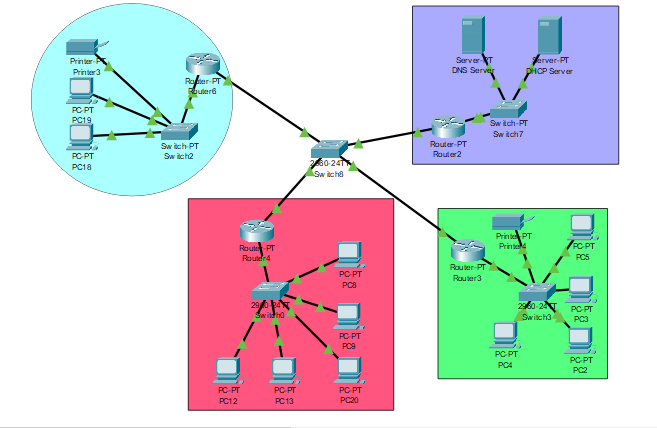
\includegraphics[scale=0.6]{diagram.png}
			\end{center}
			\textbf{Note :} untuk bentuk diagramnya bebas boleh membuat berbagai macam variasi, begitu juga dengan pengalamatan IP, boleh memakai variasi address apapun

			\item \textbf{Buatlah video singkat berdurasi 5-7 menit berisi penjelasan singkat terkait diagram jaringan yang praktikan buat. Diharapkan seluruh anggota kelompok memiliki peran dalam menjelaskan diagram yang dibuat.} 
		\end{itemize}
	\end{flushleft}
	
	\newpage

	\begin{center}
        \textbf{Question}
    \end{center}
	
    \begin{itemize}
    	\item Menurut anda, prefix apakah yang cocok untuk jaringan kantor tersebut (jawaban bersifat bebas menurut praktikan) ?
    	\item Tuliskan Network Address untuk masing-masing keempat ruangan dan Network yang menghubungkan antar Router ? (Buat listnya)
    \end{itemize}
\end{document}
